%!TEX root = ../Thesis.tex

\section{Effect of adapting the variance}\label{sec: Experimental work: Effect of adapting the variance}
Until now, all experiments have been run with an isotropic Gaussian with fixed variance similarly to \cite{Salimans2017}. Here, different variants of the Gaussian search distribution with adaptive variance will be examined.
The examined variants are the isotropic Gaussian, the layer-wise separable Gaussian and the parameter-wise separable Gaussian. For the layer-wise separable Gaussian, a single variance parameter is used for each weight/kernel matrix and bias vector in the model.
Hyperparameters are otherwise as in \autoref{sec: Experimental work: Effects of common model and algorithm augmentations}.

For these experiments, a momentum of $0.9$ has been used on the parameter gradient as well as the adapted variance gradient while the variance gradient is also dampened by $0.9$. Dampening the variance gradient makes sure it does not spike as discussed in \autoref{sec: Experimental work: Effect of momentum}. Dampened momentum on the variance gradient results in much smoother updates to the variance than applying no momentum or non-dampened momentum. Learning rates of $2$ and $4$ have been used for the isotropic and separable Gaussian variances, respectively.


\subsection{Adapting the variance}
\autoref{fig: Theory: E029-VO-S5-MD-analysis} shows the results of running the \gls{VO} algorithm on the MNIST network with the different search distributions. 
\autoref{fig: Theory: E029-VO-S5-MD-analysis/accuracy_val-all-series-mean-sd} and \ref{fig: Theory: E029-VO-S5-MD-analysis/return_val-all-series-mean-sd} respectively show the validation set accuracy and \gls{NLL} loss for the different search distributions.
The most notable difference between the variations is that when the variance is adapted, the isotropic Gaussian gives somewhat unstable learning, in that it gives quite different results solely dependent on random seed.
This can be seen not to be the case when adapting a layer- or parameter-wise separable Gaussians. 

Despite this, the convergence rate and the median final \gls{NLL} loss and accuracy are not improved when using these adaptive search distributions compared to using the fixed isotropic Gaussian. 
Considering the single best and worst performing models on the validation set, it can be noted that these are all obtained by the separable versions. As such, adapting the variance seems to encourage more extensive exploration of the loss landscape but with risk of landing in both a slightly better and slightly worse minimum than would have been reached with a fixed variance.

It should be noted that these observations hold for many different learning rates for the variance parameter(s).

\begin{figure}[tbp!]
    \begin{subfigure}[b]{0.49\textwidth}
        \centering
        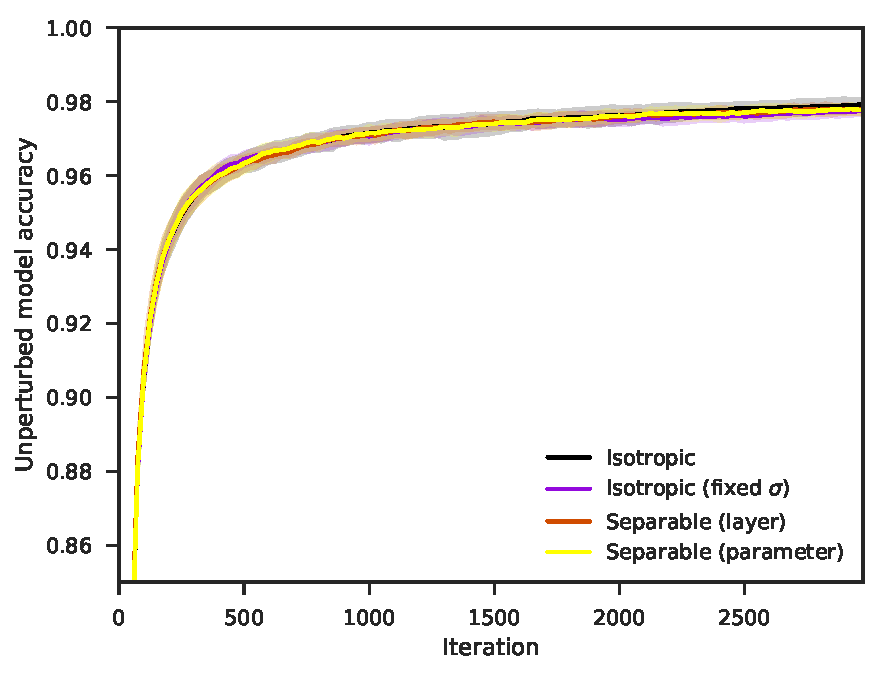
\includegraphics[height=5.8cm]{graphics/E029-VO-S5-MD-analysis/accuracy_val-all-series-mean-sd.pdf}
        \caption{}
        \label{fig: Theory: E029-VO-S5-MD-analysis/accuracy_val-all-series-mean-sd}
    \end{subfigure}
    \hfill
    \begin{subfigure}[b]{0.49\textwidth}
        \centering
        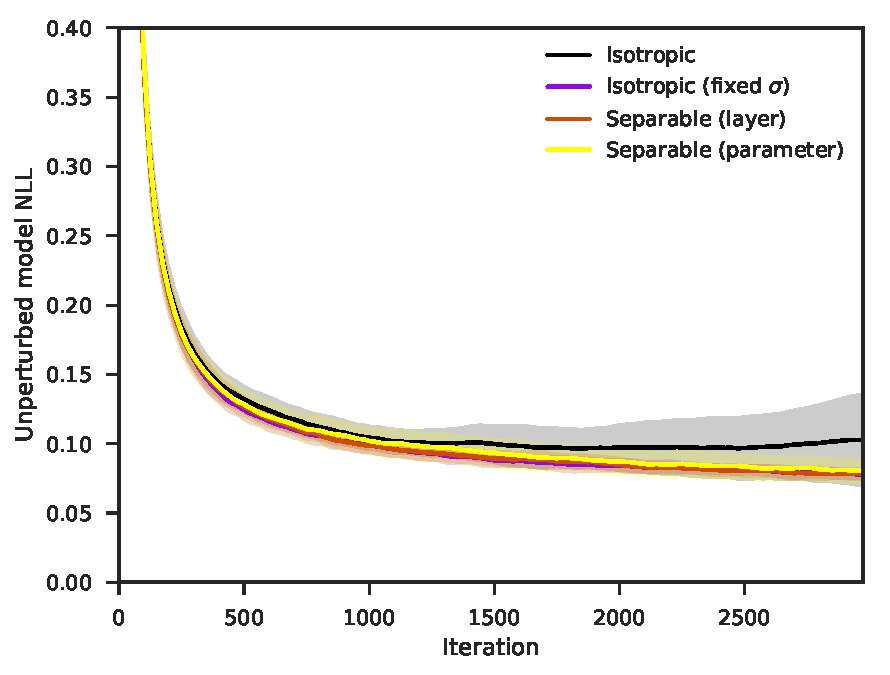
\includegraphics[height=5.8cm]{graphics/E029-VO-S5-MD-analysis/return_val-all-series-mean-sd.pdf}
        \caption{}
        \label{fig: Theory: E029-VO-S5-MD-analysis/return_val-all-series-mean-sd}
    \end{subfigure}
    \begin{subfigure}[b]{0.49\textwidth}
        \centering
        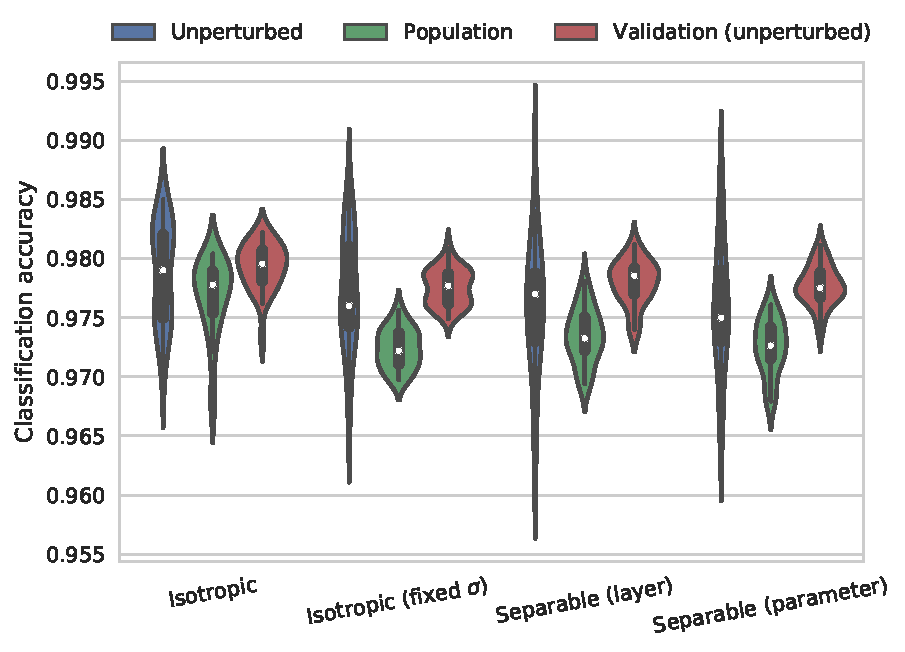
\includegraphics[height=5.3cm]{graphics/E029-VO-S5-MD-analysis/accuracy-final-distribution-boxplot-grouped.pdf}
        \caption{}
        \label{fig: Theory: E029-VO-S5-MD-analysis/accuracy-final-distribution-boxplot-grouped}
    \end{subfigure}
    \hfill
    \begin{subfigure}[b]{0.49\textwidth}
        \centering
        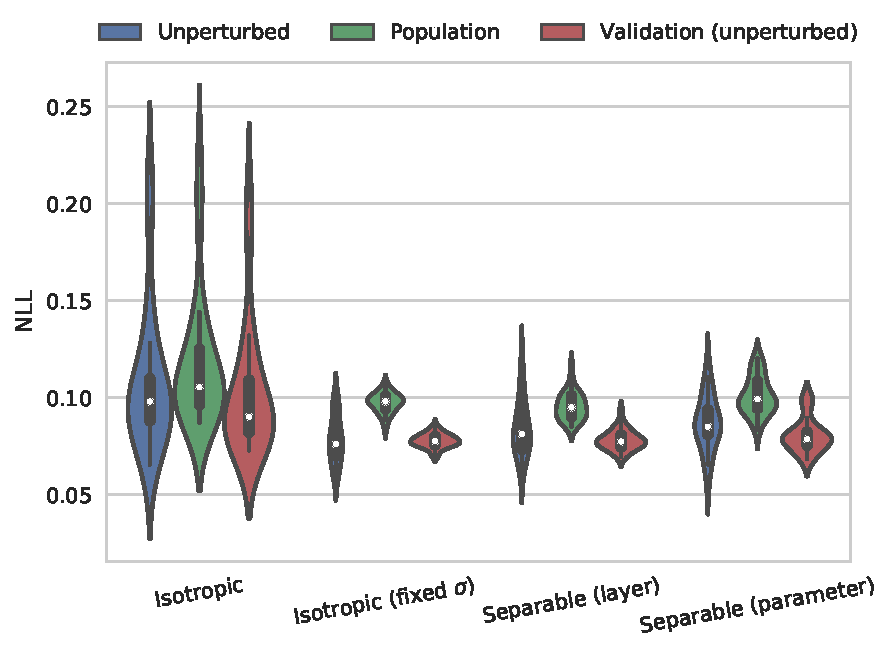
\includegraphics[height=5.3cm]{graphics/E029-VO-S5-MD-analysis/return-final-distribution-boxplot-grouped.pdf}
        \caption{}
        \label{fig: Theory: E029-VO-S5-MD-analysis/return-final-distribution-boxplot-grouped}
    \end{subfigure}
    \caption{
        Results of experiments with different \gls{VO} algorithms. The model variations are the fixed variance strategy of \cite{Salimans2017} and \gls{VO} with adjusted variance using an isotropic Gaussian and respectively a layer-wise and per-weight separable Gaussian. Contrary to \cite{Salimans2017}, safe mutation is applied.
        Plotted versus the iteration number, \subref{fig: Theory: E029-VO-S5-MD-analysis/accuracy_val-all-series-mean-sd} shows the validation set classification accuracy and \subref{fig: Theory: E029-VO-S5-MD-analysis/return_val-all-series-mean-sd} the validation set \gls{NLL} loss. 
        Difference in performance between the algorithms is very small and within one standard deviation with the adapted isotropic having high between-run variance.
        In \subref{fig: Theory: E029-VO-S5-MD-analysis/accuracy-final-distribution-boxplot-grouped} and \subref{fig: Theory: E029-VO-S5-MD-analysis/return-final-distribution-boxplot-grouped} the final distribution of the classification accuracy and \gls{NLL} loss from \subref{fig: Theory: E029-VO-S5-MD-analysis/accuracy_val-all-series-mean-sd} and \subref{fig: Theory: E029-VO-S5-MD-analysis/return_val-all-series-mean-sd} are shown. It can be noted that adapting the variance in the isotropic Gaussian search distribution results a much wider span of the final \gls{NLL} loss. Additionally, a small group of runs has an even higher final \gls{NLL} loss than the main body of runs. This is not observed for the other versions.
        %These seem to hint at a potential better final performance by adapting the variance of a layer-wise separable Gaussian search distribution.
        %which is more flexible than an isotropic Gaussian but has fewer parameters and is easier to estimate than a separable Gaussian with per-weight variances.
    }
    \label{fig: Theory: E029-VO-S5-MD-analysis}
\end{figure}


% \begin{figure}[tbp!]
%     \begin{subfigure}[b]{0.49\textwidth}
%         \centering
%         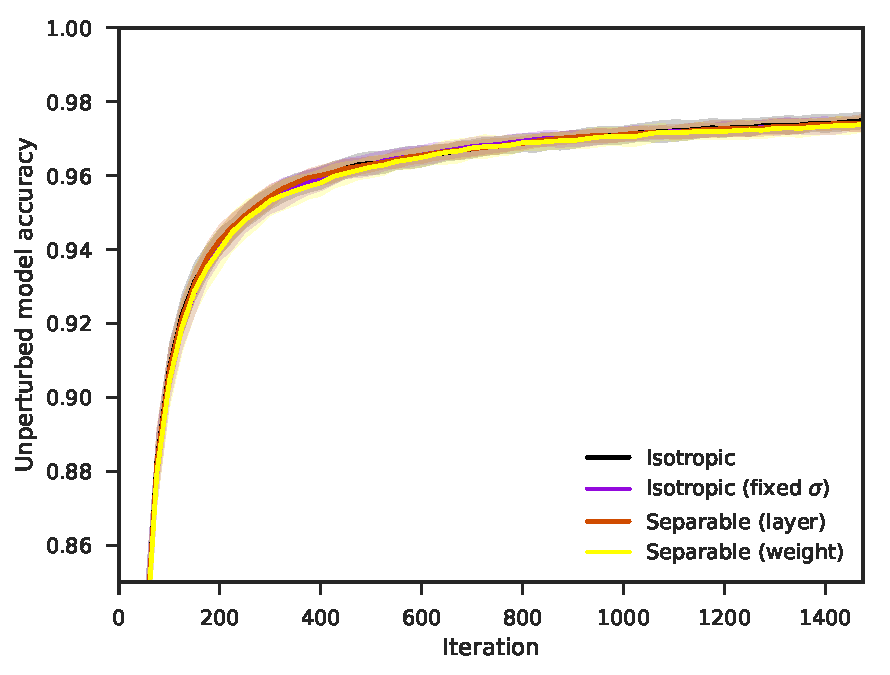
\includegraphics[height=5.8cm]{graphics/E029-VO-S3-analysis-1500/accuracy_val-all-series-mean-sd.pdf}
%         \caption{}
%         \label{fig: Theory: E029-VO-S3-analysis-1500/accuracy_val-all-series-mean-sd}
%     \end{subfigure}
%     \hfill
%     \begin{subfigure}[b]{0.49\textwidth}
%         \centering
%         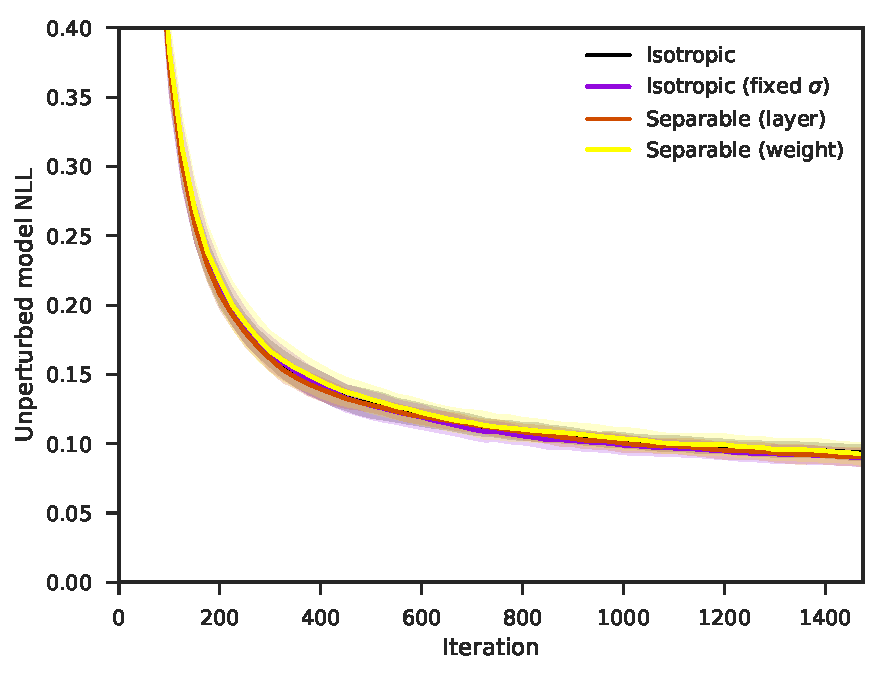
\includegraphics[height=5.8cm]{graphics/E029-VO-S3-analysis-1500/return_val-all-series-mean-sd.pdf}
%         \caption{}
%         \label{fig: Theory: E029-VO-S3-analysis-1500/return_val-all-series-mean-sd}
%     \end{subfigure}
%     \begin{subfigure}[b]{0.49\textwidth}
%         \centering
%         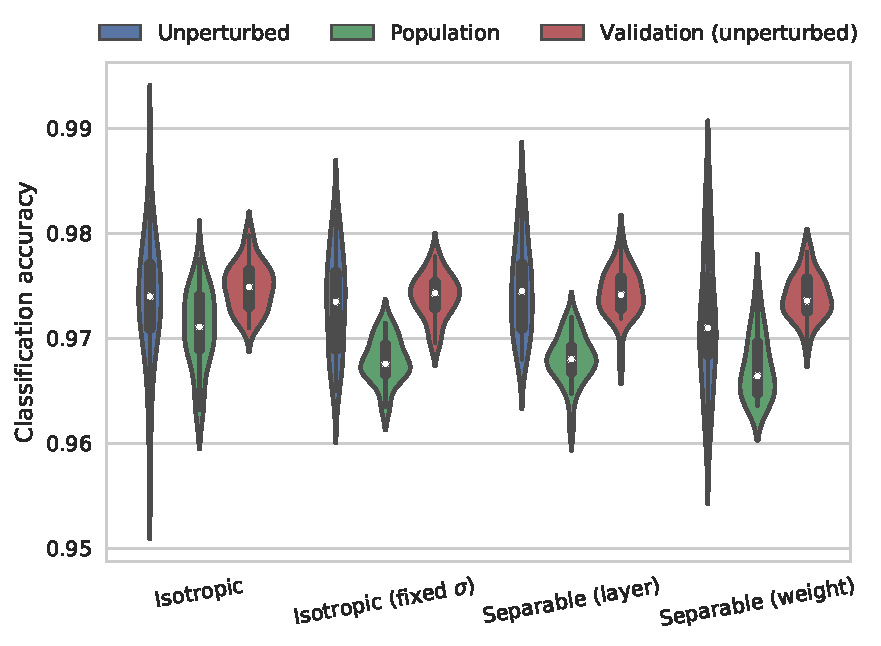
\includegraphics[height=5.3cm]{graphics/E029-VO-S3-analysis-1500/accuracy-final-distribution-boxplot-grouped.pdf}
%         \caption{}
%         \label{fig: Theory: E029-VO-S3-analysis-1500/accuracy-final-distribution-boxplot-grouped}
%     \end{subfigure}
%     \hfill
%     \begin{subfigure}[b]{0.49\textwidth}
%         \centering
%         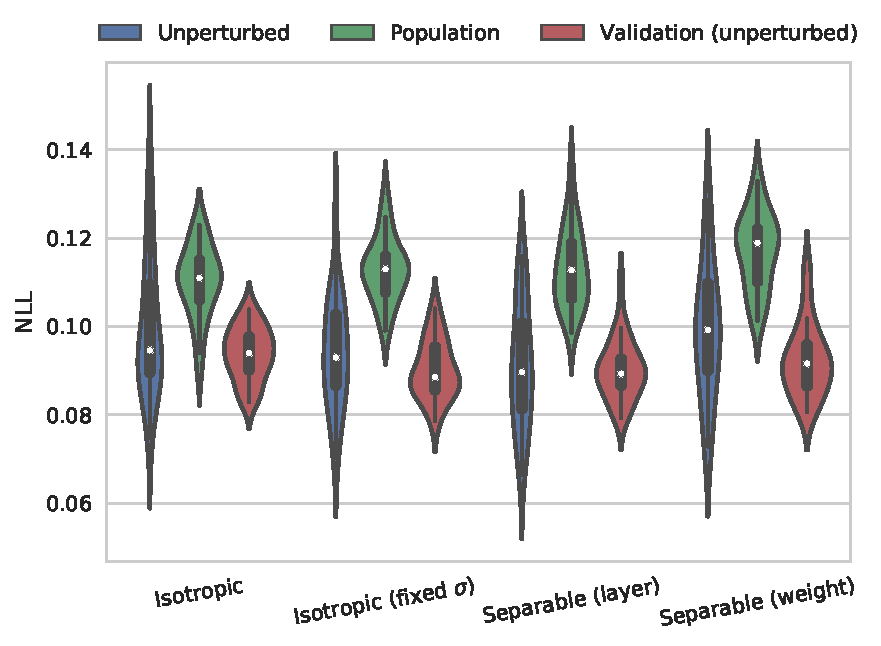
\includegraphics[height=5.3cm]{graphics/E029-VO-S3-analysis-1500/return-final-distribution-boxplot-grouped.pdf}
%         \caption{}
%         \label{fig: Theory: E029-VO-S3-analysis-1500/return-final-distribution-boxplot-grouped}
%     \end{subfigure}
%     \caption{
%         Results of experiments with different \gls{VO} algorithms. The model variations are the fixed variance strategy of \cite{Salimans2017} and \gls{VO} with adjusted variance using an isotropic Gaussian and respectively a layer-wise and per-weight separable Gaussian. Contrary to \cite{Salimans2017}, safe mutation is applied.
%         Plotted versus the iteration number \subref{fig: Theory: E029-VO-S3-analysis-1500/accuracy_val-all-series-mean-sd} shows the validation set classification accuracy and \subref{fig: Theory: E029-VO-S3-analysis-1500/return_val-all-series-mean-sd} the validation set \gls{NLL} loss. 
%         Difference in performance between the algorithms is very small and certainly insignificant.
%         In \subref{fig: Theory: E029-VO-S3-analysis-1500/accuracy-final-distribution-boxplot-grouped} and \subref{fig: Theory: E029-VO-S3-analysis-1500/return-final-distribution-boxplot-grouped} the final distribution of the classification accuracy and \gls{NLL} loss from \subref{fig: Theory: E029-VO-S3-analysis-1500/accuracy_val-all-series-mean-sd} and \subref{fig: Theory: E029-VO-S3-analysis-1500/return_val-all-series-mean-sd} are shown.
%         %These seem to hint at a potential better final performance by adapting the variance of a layer-wise separable Gaussian search distribution.
%         %which is more flexible than an isotropic Gaussian but has fewer parameters and is easier to estimate than a separable Gaussian with per-weight variances.
%     }
%     \label{fig: Theory: E029-VO-S3-analysis-1500}
% \end{figure}


% \begin{figure}[tbp!]
%     \begin{subfigure}[b]{0.49\textwidth}
%         \centering
%         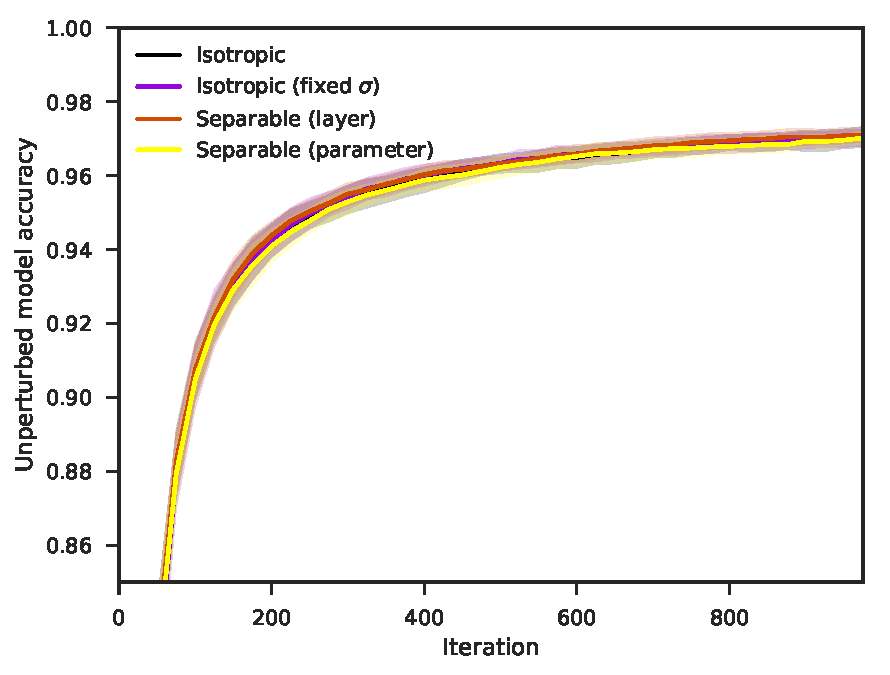
\includegraphics[height=5.8cm]{graphics/E029-VO-S2-analysis/accuracy_val-all-series-mean-sd.pdf}
%         \caption{}
%         \label{fig: Theory: E029-VO-S2-analysis/accuracy_val-all-series-mean-sd}
%     \end{subfigure}
%     \hfill
%     \begin{subfigure}[b]{0.49\textwidth}
%         \centering
%         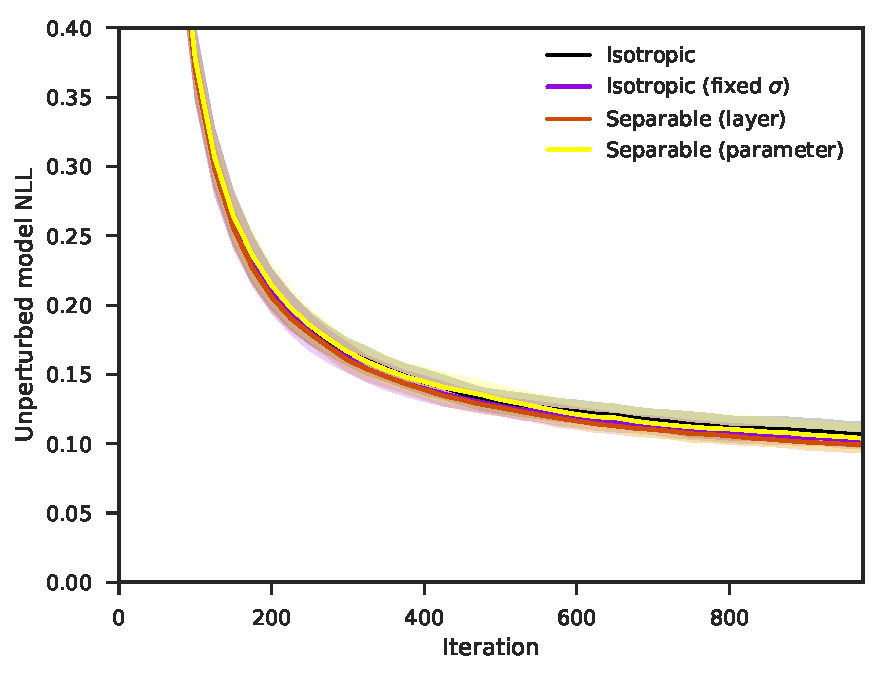
\includegraphics[height=5.8cm]{graphics/E029-VO-S2-analysis/return_val-all-series-mean-sd.pdf}
%         \caption{}
%         \label{fig: Theory: E029-VO-S2-analysis/return_val-all-series-mean-sd}
%     \end{subfigure}
%     \begin{subfigure}[b]{0.49\textwidth}
%         \centering
%         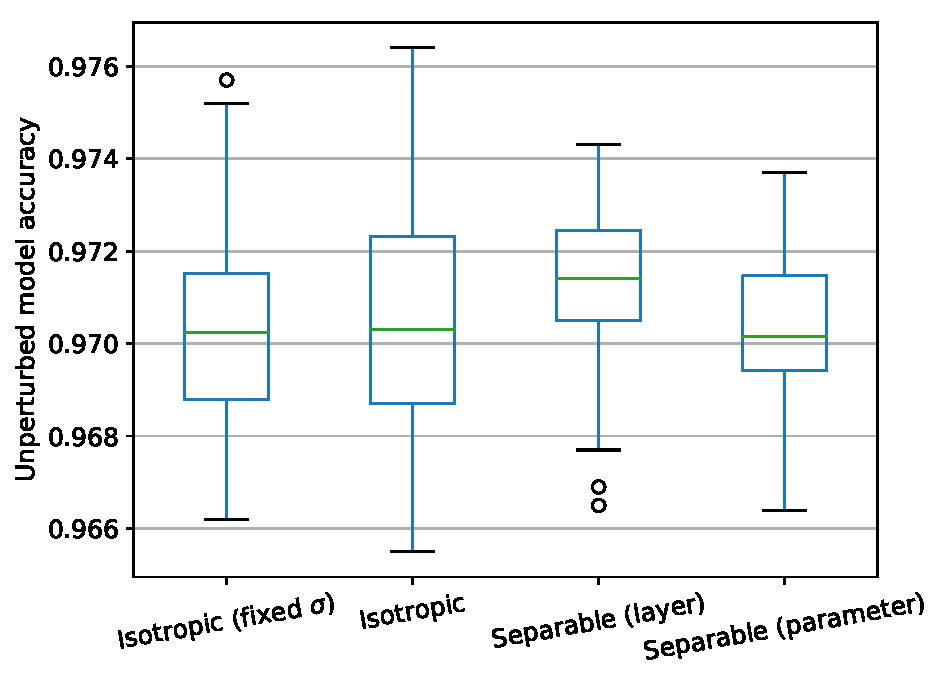
\includegraphics[height=5.2cm]{graphics/E029-VO-S2-analysis/accuracy_val-final-distribution-boxplot.pdf}
%         \caption{}
%         \label{fig: Theory: E029-VO-S2-analysis/accuracy_val-final-distribution-boxplot}
%     \end{subfigure}
%     \hfill
%     \begin{subfigure}[b]{0.49\textwidth}
%         \centering
%         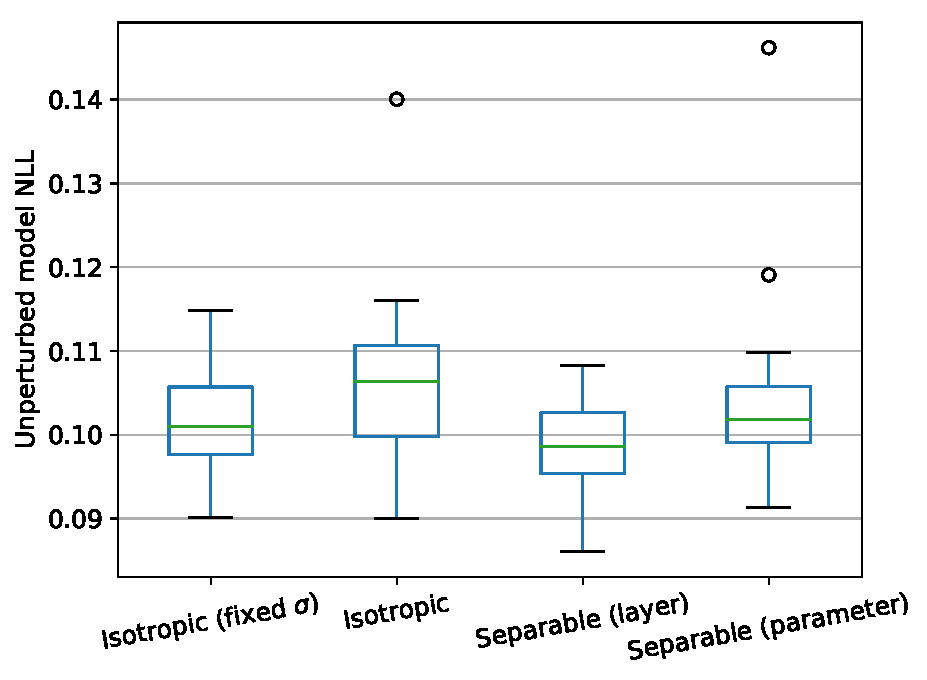
\includegraphics[height=5.2cm]{graphics/E029-VO-S2-analysis/return_val-final-distribution-boxplot.pdf}
%         \caption{}
%         \label{fig: Theory: E029-VO-S2-analysis/return_val-final-distribution-boxplot}
%     \end{subfigure}
%     \caption{
%         Results of experiments with different \gls{VO} algorithms. The plots all show the validation \gls{NLL} or the validation classification accuracy of the unperturbed model. The model variations are the fixed variance strategy of \cite{Salimans2017} and \gls{VO} with adjusted variance using an isotropic Gaussian and respectively a layer-wise and per-weight separable Gaussian.
%         Plotted versus the iteration number \subref{fig: Theory: E029-VO-S2-analysis/accuracy_val-all-series-mean-sd} shows the validation set classification accuracy and \subref{fig: Theory: E029-VO-S2-analysis/return_val-all-series-mean-sd} the validation set \gls{NLL} loss. Difference in performance between the algorithms is very small and certainly insignificant.
%         In \subref{fig: Theory: E029-VO-S2-analysis/accuracy_val-final-distribution-boxplot} and \subref{fig: Theory: E029-VO-S2-analysis/return_val-final-distribution-boxplot} the final distribution of the classification accuracy and \gls{NLL} loss from \subref{fig: Theory: E029-VO-S2-analysis/accuracy_val-all-series-mean-sd} and \subref{fig: Theory: E029-VO-S2-analysis/return_val-all-series-mean-sd} are shown. These seem to hint at a potential better final performance by adapting the variance of a layer-wise separable Gaussian search distribution.
%         %which is more flexible than an isotropic Gaussian but has fewer parameters and is easier to estimate than a separable Gaussian with per-weight variances.
%     }
%     \label{fig: Theory: E029-VO-S2-analysis}
% \end{figure}







\subsection{The gradient norm}
This section examines the interaction between adapting the variance and the norm of the \gls{VO} gradient and the parameter vector in order to shed more light on the effect of adapting the variance. It does so based on single runs of the training, but it should be noted that the observations hold generally for additional runs with different random seeds.

Consider the gradient and parameter norms when using an isotropic Gaussian search distribution. 
As can be seen from the derived \gls{VO} gradient estimators in \eqref{eq: Theory: Variational optimization multivariate isotropic gaussian gradient estimators}, the gradient is scaled by the variance.
In case the variance is fixed, this is obviously a constant scaling factor.
However, when adapting the variance, this effectively scales the term computed by the sum differently at each iteration. It is evident that the variance then has a direct adaptive effect on the gradient norm and thus affects the iteration step size. The effect that the variance has through multiplication on the perturbation and indirectly through the value of the objective function is harder to determine. Since the perturbations are from a standard Gaussian, multiplying them by $\sigma$ does not change their expectation. Additionally, it is theoretically possible for the objective function to both increase and decrease in value for any size of the perturbation. However, very large perturbations must be expected to result in catastrophic forgetting in the perturbed networks as any learned filters etc. are washed out with noise.

\begin{figure}[tbp!]
    \begin{subfigure}[b]{0.49\textwidth}
        \centering
        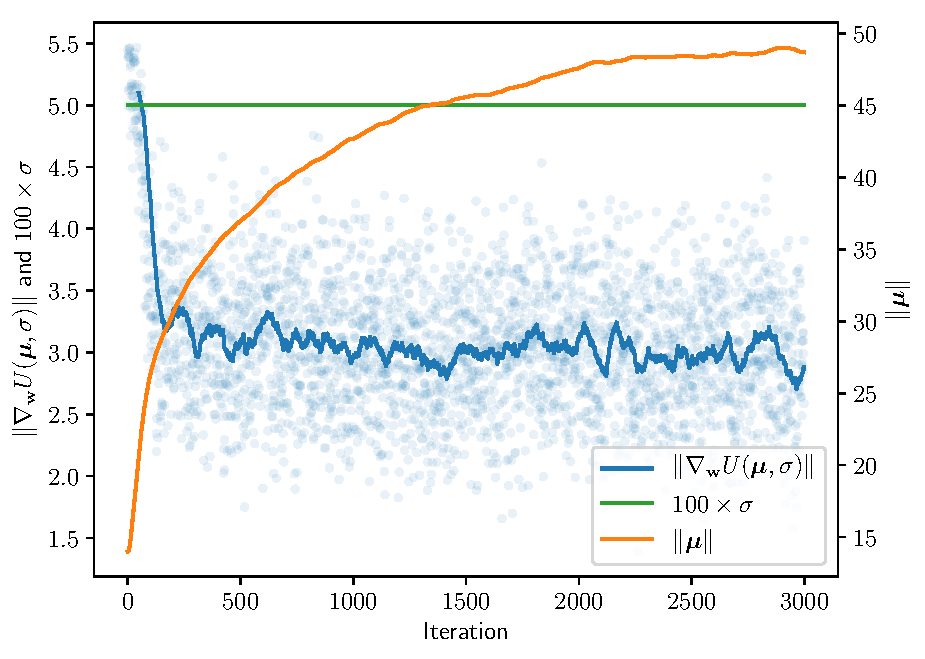
\includegraphics[height=5.5cm]{graphics/E031-NORM-analysis/isotropic-fixed-1-param-and-grad-and-variance-norm.pdf}
        \caption{}
        \label{fig: Theory: E031-NORM-analysis/isotropic-fixed-1-param-and-grad-and-variance-norm}
    \end{subfigure}
    \hfill
    \begin{subfigure}[b]{0.49\textwidth}
        \centering
        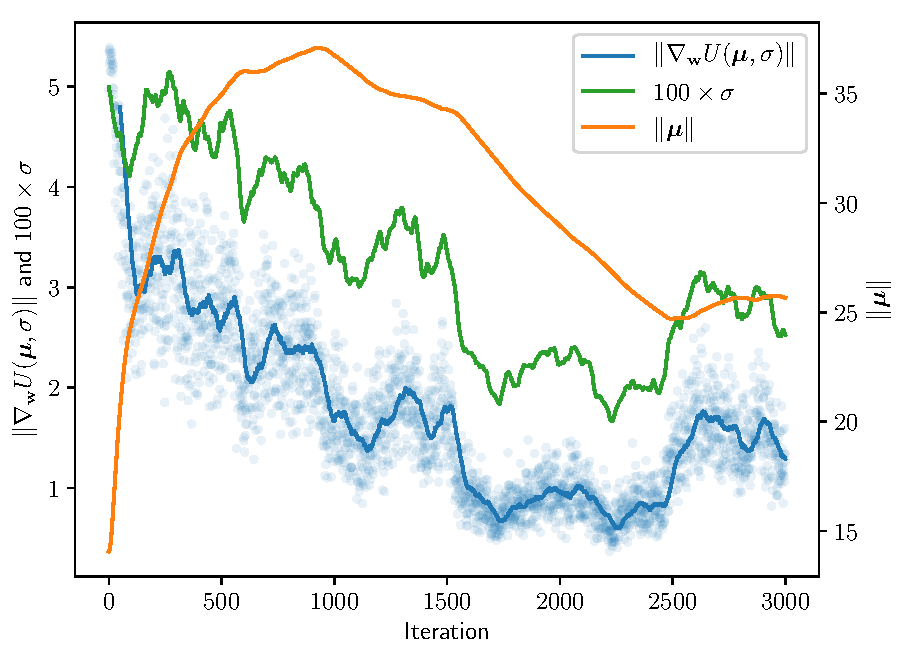
\includegraphics[height=5.5cm]{graphics/E031-NORM-analysis/isotropic-adapted-1-param-and-grad-and-variance-norm.pdf}
        \caption{}
        \label{fig: Theory: E031-NORM-analysis/isotropic-adapted-1-param-and-grad-and-variance-norm}
    \end{subfigure}
    \caption{
        2-norms of the \gls{NN} parameter vector and \gls{VO} gradient for an isotropic Gaussian search distribution with the variance overlayed (multiplied by 100 for scale). In \subref{fig: Theory: E031-NORM-analysis/isotropic-fixed-1-param-and-grad-and-variance-norm} and \subref{fig: Theory: E031-NORM-analysis/isotropic-adapted-1-param-and-grad-and-variance-norm}, the fixed and adapted variance versions are shown, respectively. A centered $50$ sample moving average is computed for the gradient. It is clear that adapting the variance directly and significantly influences the norm of the gradient and in turn also the norm of the parameter vector.
    }
    \label{fig: Theory: E031-NORM-analysis-isotropic}
\end{figure}
The gradient and parameter norms for fixed and adapted variance isotropic Gaussians are plotted in \autoref{fig: Theory: E031-NORM-analysis-isotropic} for a single run of the \gls{MNIST} network (\autoref{lst: Network models: MNIST with batch normalization}). The variance is overlaid in the plots as well. 
A fixed variance (\ref{fig: Theory: E031-NORM-analysis/isotropic-fixed-1-param-and-grad-and-variance-norm}) results in a gradient that rapidly reaches a constant level. The parameter norm increases fairly steadily as a result, but seems to plateau when a minimum is found\footnote{The learning curves are similar to the ones in \autoref{fig: Theory: E029-VO-S5-MD-analysis}}. Interestingly enough, the gradient does not go to zero as the minimum is reached but remains relatively high. This is in-line with the rarity of local minima and the prevalence of saddle points as previously mentioned.
It should be noted that the small amount of $L^2$ regularization adds to decrease the parameter norm. By adapting the variance (\ref{fig: Theory: E031-NORM-analysis/isotropic-adapted-1-param-and-grad-and-variance-norm}), the gradient is also adapted: As the variance decreases so does the gradient norm and in turn the parameter norm as well. The effect of the variance on the gradient norm is similar to that of adaptively decreasing the learning rate during training in the way that increasingly smaller steps are taken as training progresses. By inspecting the results presented in \autoref{fig: Theory: E029-VO-S5-MD-analysis}, it was found that the small poorly performing group of runs that used the adapted isotropic Gaussian had a variance that generally increased rather than decreased throughout training. This then directly resulted in larger gradients and in turn divergence.

\begin{figure}[tbp!]
    \begin{subfigure}[b]{0.49\textwidth}
        \centering
        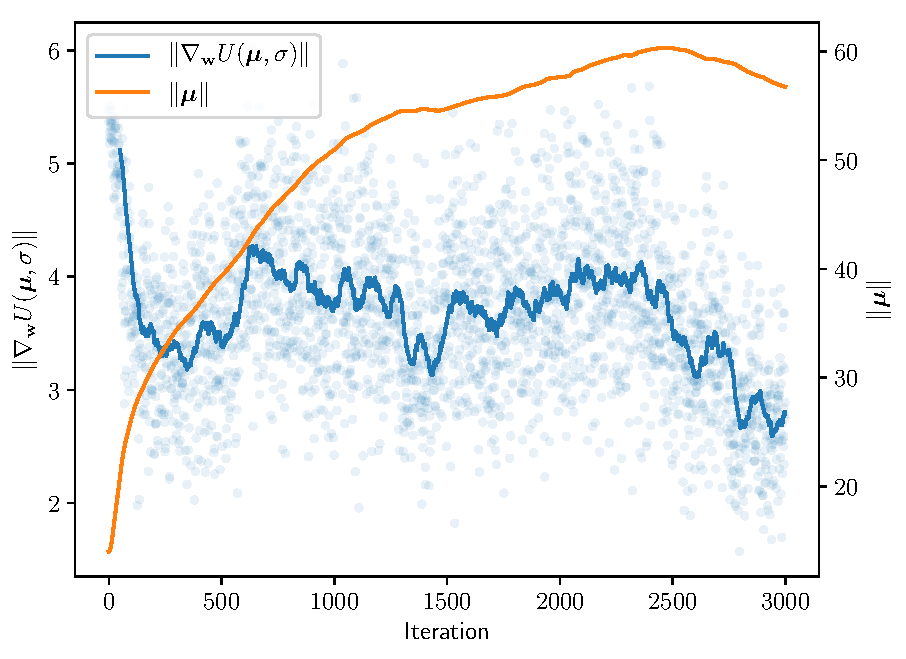
\includegraphics[height=5.6cm]{graphics/E031-NORM-analysis/separable-layer-5-param-and-grad-norm.pdf}
        \caption{}
        \label{fig: Theory: E031-NORM-analysis/separable-layer-5-param-and-grad-norm}
    \end{subfigure}
    \hfill
    \begin{subfigure}[b]{0.49\textwidth}
        \centering
        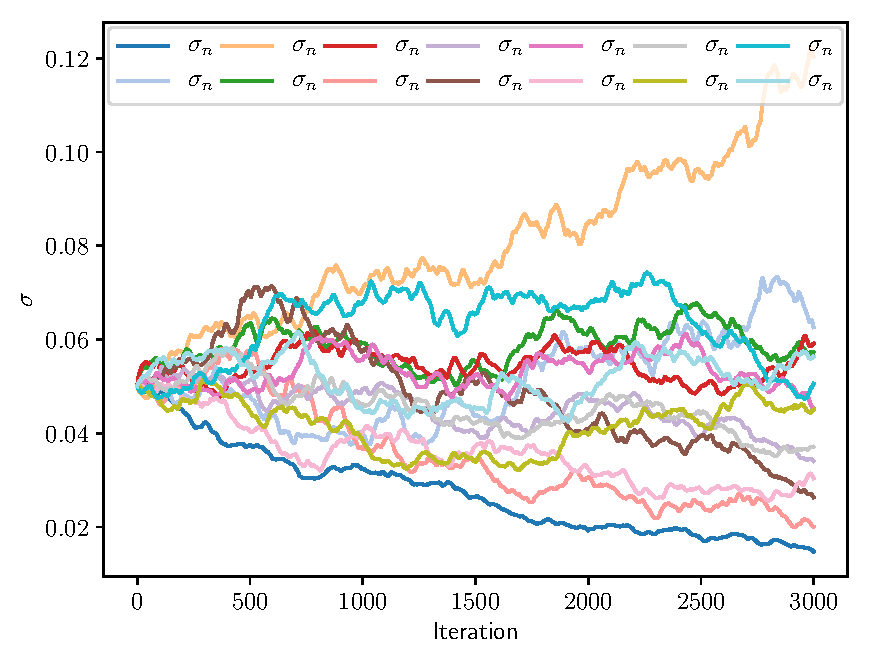
\includegraphics[height=5.6cm]{graphics/E031-NORM-analysis/separable-layer-5-variance.pdf}
        \caption{}
        \label{fig: Theory: E031-NORM-analysis/separable-layer-5-variance}
    \end{subfigure}
    \caption{
        \subref{fig: Theory: E031-NORM-analysis/separable-layer-5-param-and-grad-norm} 2-norms of the \gls{NN} parameter vector and \gls{VO} gradient for a layer-wise separable Gaussian search distribution with the variances plotted separately in \subref{fig: Theory: E031-NORM-analysis/separable-layer-5-variance}. Most variances tend to zero while a few increase. The gradient norm feels the combined effect but generally increases.
    }
    \label{fig: Theory: E031-NORM-analysis-layer-separable}
\end{figure}
\begin{table}[!tbp]
    \centering
    \begin{tabular}{llcc}
\toprule
\# & Layer  & weight/kernel & bias\\
\midrule
1 & Convolutional         &  0  &  1\\
2 & Batch normalization   &  2  &  3\\
3 & Convolutional         &  4  &  5\\
4 & Batch normalization   &  6  &  7\\
5 & Fully connected       &  8  &  9\\
6 & Batch normalization   &  10  &  11\\
7 & Fully connected       &  12  &  13\\
\bottomrule
    \end{tabular}
    \caption{Labels of the variances of the layer-wise separable Gaussian in \autoref{fig: Theory: E031-NORM-analysis-layer-separable} used on the \gls{MNIST} model in \autoref{lst: Network models: MNIST with batch normalization}. The labels are divided into those for the weight/kernel and those for the bias.}
    \label{tab: Experimental work: Adapting the variance}
\end{table}

For the layer-wise separable Gaussians, \autoref{fig: Theory: E031-NORM-analysis-layer-separable} shows the results.
Here, the variances are plotted separately for clarity. 
The variances are labelled incrementally by their layer in the model as described by \autoref{tab: Experimental work: Adapting the variance}. This search distribution often sees many of the variances go toward zero while a few increase.
As for the isotropic case the gradient norm is influenced, but now depends on all the variances. As such it is slightly more smooth but also does not trend as clearly to zero.
One can note that there is some tendency for the variances of earlier layers to decrease more than for later layers. Specifically, the three variances that increase the most are for the \nth{7}, \nth{6} and \nth{5} layer. This can be speculated to be due to the features of earlier layers being learned sooner during training than features of later layers. This might then result in flatter regions of the loss surface in the respective dimensions and thus decreasing variances.

\begin{figure}[tbp!]
    \begin{subfigure}[b]{0.49\textwidth}
        \centering
        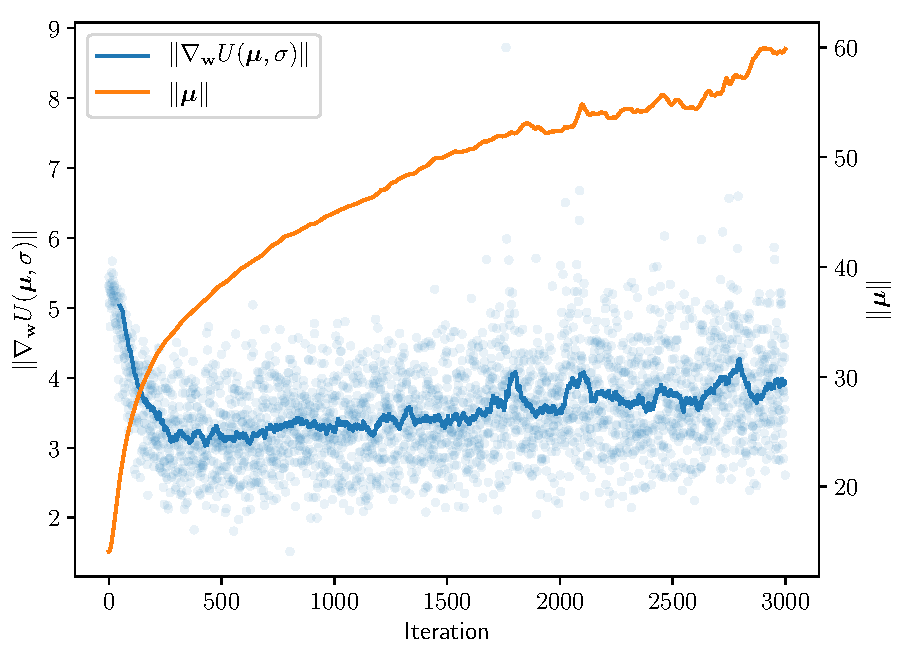
\includegraphics[height=5.6cm]{graphics/E031-NORM-analysis/separable-parameter-1-param-and-grad-norm.pdf}
        \caption{}
        \label{fig: Theory: E031-NORM-analysis/separable-parameter-1-param-and-grad-norm}
    \end{subfigure}
    \hfill
    \begin{subfigure}[b]{0.49\textwidth}
        \centering
        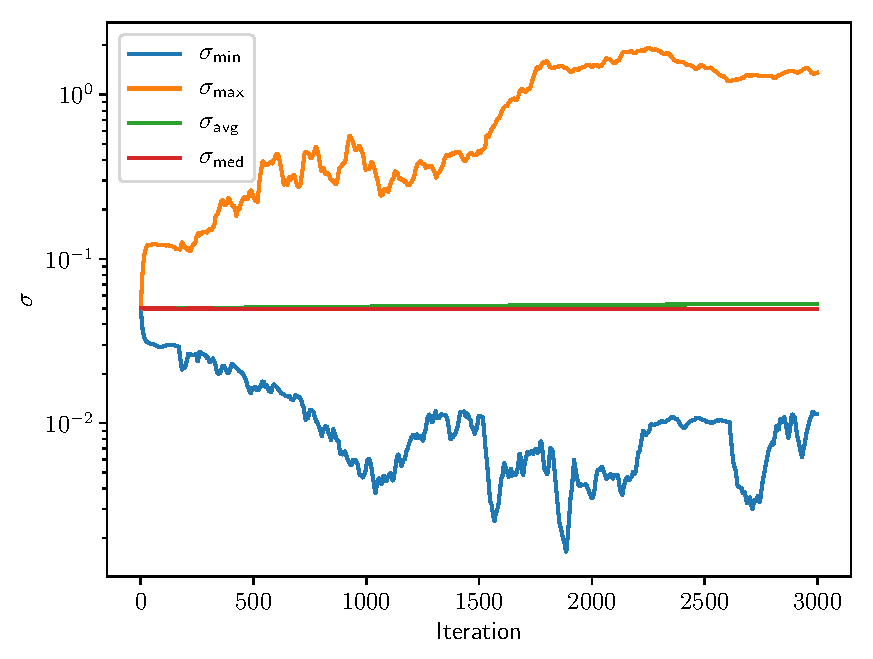
\includegraphics[height=5.6cm]{graphics/E031-NORM-analysis/separable-parameter-1-variance.pdf}
        \caption{}
        \label{fig: Theory: E031-NORM-analysis/separable-parameter-1-variance}
    \end{subfigure}
    \caption{
        \subref{fig: Theory: E031-NORM-analysis/separable-parameter-1-param-and-grad-norm} 2-norms of the \gls{NN} parameter vector and \gls{VO} gradient for a parameter-wise separable Gaussian search distribution with the maximal, minimal, average and median variances plotted separately in \subref{fig: Theory: E031-NORM-analysis/separable-parameter-1-variance}.
    }
    \label{fig: Theory: E031-NORM-analysis-parameter-separable}
\end{figure}
The variances of the parameter-wise separable Gaussian behave similar to the variances of the layer-wise but in a more extreme way and are shown in \autoref{fig: Theory: E031-NORM-analysis-parameter-separable}. The maximal and minimal variances change by two orders of magnitude while the median and average variances remain close to the initial value of $0.5$. The effect on the gradient norm is smaller but there is a tendency for it to increase compared to the fixed variance isotropic Gaussian in \autoref{fig: Theory: E031-NORM-analysis/isotropic-fixed-1-param-and-grad-and-variance-norm}. 
That the parameter-wise variances tend to both increase and decrease by potentially large amounts while the average and median remain approximately at the initial value may indicate that the behaviour is similar to a random walk. 
This behaviour may be due to the fact that many more variance gradients need to be estimated at each iteration while using the same number of perturbations. Additionally, the gradient of the variance of an isotropic Gaussian is estimated by computing the sum of squares of all elements of each perturbation vector. This holds as well for each variance of a layer-wise separable Gaussian considering only the elements used for each layer. In the parameter-wise case however, a single contribution is made from each element of a perturbation vector.
As such, the reason for the random walk behaviour of the variances may be attributable to a poor estimate of their gradients due to a number of effective samples that is too low.


\subsection{Discussion}
The trends in the values of the adapted variances of the separable Gaussians seem to indicate that different layers/parameters have different optimal variances for their perturbations at different times during training. This might help explain why adapting the variance for an isotropic Gaussian sometimes results in divergence while this does not happen for separable Gaussians. When using an isotropic Gaussian, the variance may not be able to appropriately adapt to a wide range of optimal perturbation sizes. Some parameters requiring low variances may then be perturbed with relatively high variance noise and risk losing learned patterns. It should be noted that this is speculative since no experiments have been performed to validate these hypotheses.

The difficulty of drawing benefit from adapting the variance of the search distribution may be partially attributable to the complex geometry of the high dimensional loss surfaces of \glspl{NN}. As previously mentioned, saddle points are exponentially more prevalent than local minima in \gls{NN} loss surfaces while a monotonically decreasing minimization path exists on the loss surface.
The \gls{VO} adapted variance attempts to zero in on a local minimum. It does so by decreasing the variance in regions of high convex curvature and increasing it in regions of low concave curvature.
While the variance is expected to go to zero at a minimum, this is not necessarily the case at a saddle point since only some dimensions exhibit convex curvature.
This is especially obvious in the case of an isotropic Gaussian since this distribution is inherently unable to parameterize differences in the variance between dimensions.
The separable Gaussians allow more such flexibility. This may be a dynamic that adds to the results observed.
Additionally, the monotonically decreasing nature of some paths along the loss surface may encourage a somewhat constant level of the variance, at least in the isotropic case.


\iffalse
Adapting sigma separable per layer seems more stable than both isotropic and per weight. May strike good compromise between flexibility and not too many parameters

How does adapting sigma relate to the shape of the loss surface?

Very steep --> decrease

Very flat --> increase

What if we never reach an area of low gradients?

How about decoupling variance size and learning rate?

\begin{enumerate}
    % \item We may already have established that natural gradient is better so maybe no need for that experiment
    % \item Vanilla ES (VO with single fixed sigma (isotropic)) with importance mixing [include batch normalization, antithetic sampling, fitness shaping and policy network weight decay for comparability]
    % \item VO with single sigma optimization (isotropic) (VO-ISO)
    % \item VO with per layer sigma optimization (separable) (VO-SEP)
    % \item VO with per weight sigma optimization (separable) (VO-SEP)
    \item VO with per layer sigma optimization (full) (VO-COV)
    \item VO with per weight sigma optimization (low rank approx for different $k$) (VO-COV)
    % \item Effect of momentum on sigma gradient (effect of optimizer examined earlier)
    % \item Baseline: back-propagated stochastic gradient descent comparison for \gls{MNIST}
\end{enumerate}

\fi








% \begin{figure}[tbp!]
%     \begin{subfigure}[b]{0.49\textwidth}
%         \centering
%         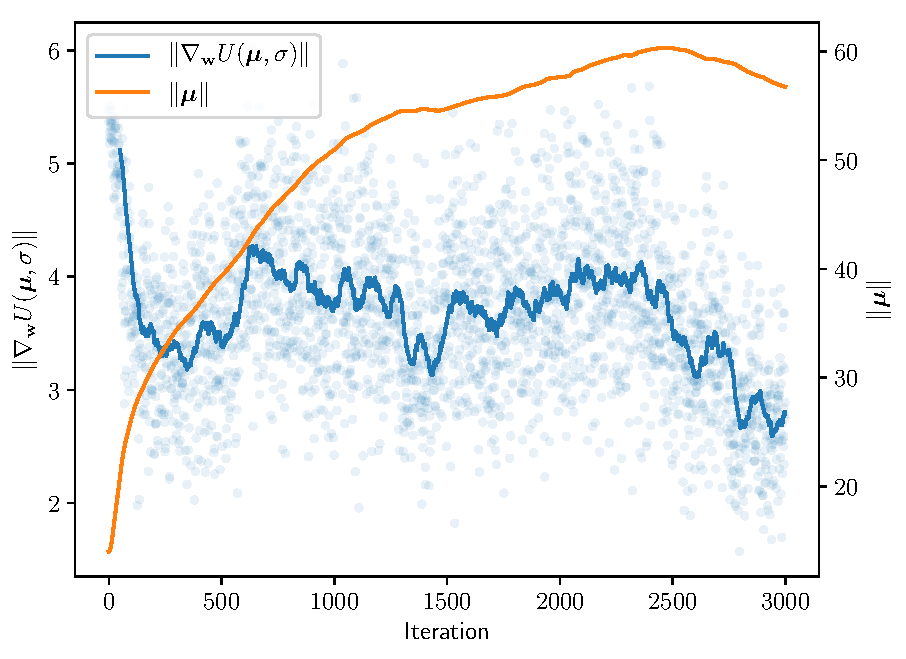
\includegraphics[height=5.6cm]{graphics/E031-NORM-analysis/separable-layer-5-param-and-grad-norm.pdf}
%         \caption{}
%         \label{fig: Theory: E031-NORM-analysis/separable-layer-5-param-and-grad-norm}
%     \end{subfigure}
%     \hfill
%     \begin{subfigure}[b]{0.49\textwidth}
%         \centering
%         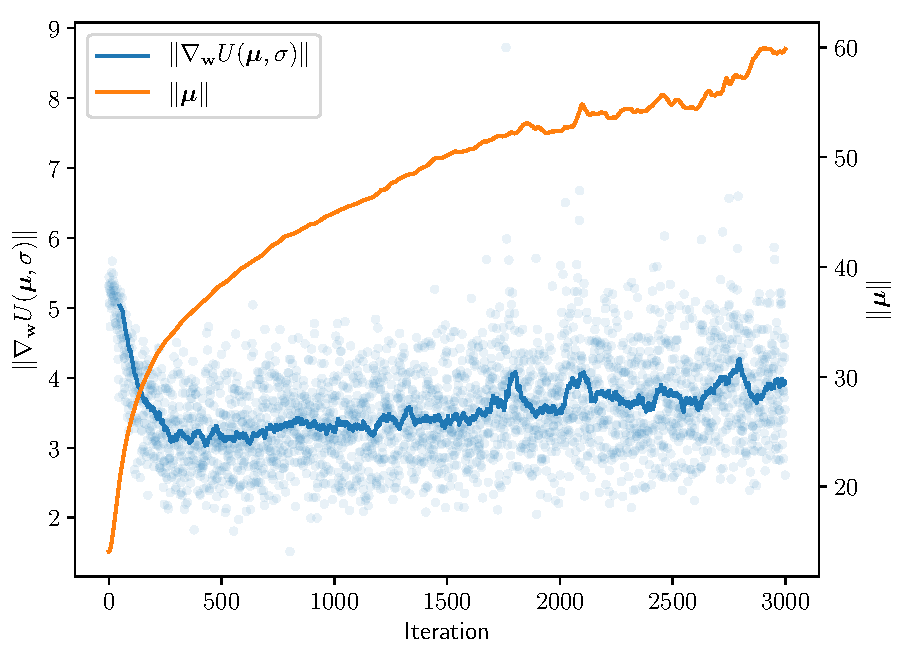
\includegraphics[height=5.6cm]{graphics/E031-NORM-analysis/separable-parameter-1-param-and-grad-norm.pdf}
%         \caption{}
%         \label{fig: Theory: E031-NORM-analysis/separable-parameter-1-param-and-grad-norm}
%     \end{subfigure}
%     \begin{subfigure}[b]{0.49\textwidth}
%         \centering
%         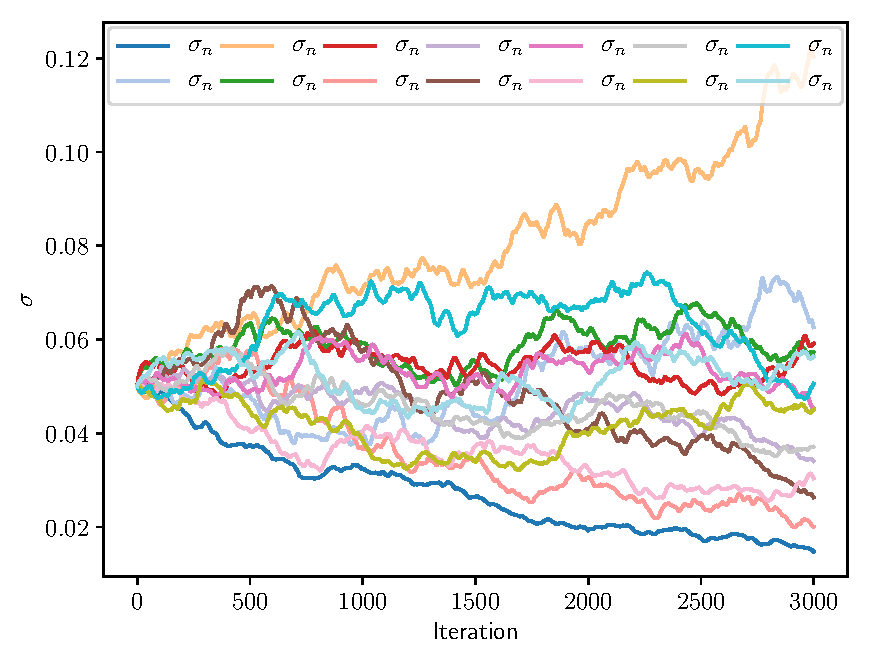
\includegraphics[height=5.8cm]{graphics/E031-NORM-analysis/separable-layer-5-variance.pdf}
%         \caption{}
%         \label{fig: Theory: E031-NORM-analysis/separable-layer-5-variance}
%     \end{subfigure}
%     \hfill
%     \begin{subfigure}[b]{0.49\textwidth}
%         \centering
%         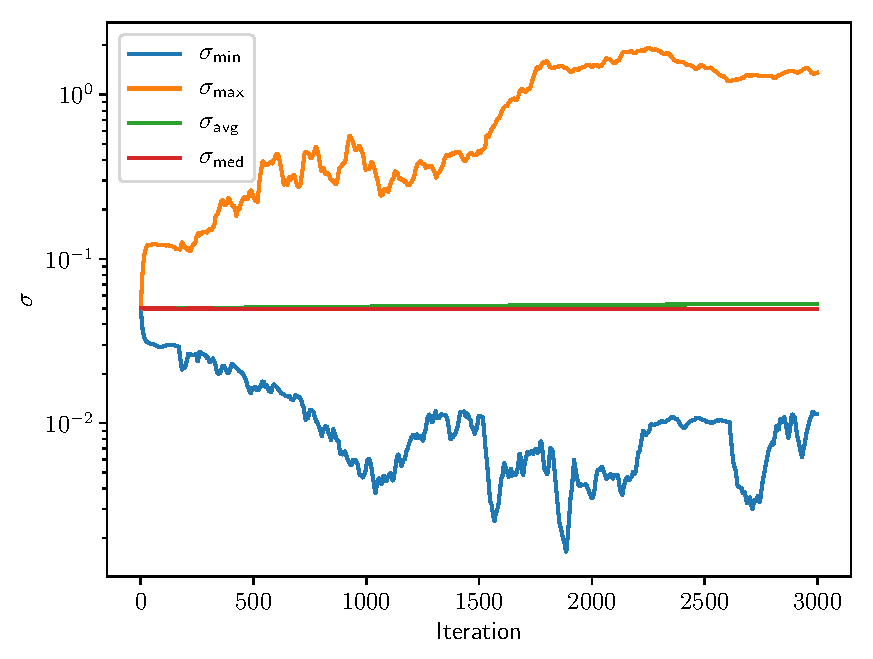
\includegraphics[height=5.8cm]{graphics/E031-NORM-analysis/separable-parameter-1-variance.pdf}
%         \caption{}
%         \label{fig: Theory: E031-NORM-analysis/separable-parameter-1-variance}
%     \end{subfigure}
%     \caption{
%         Results of experiments using \gls{SGD} with momentum on the \gls{VO} gradient for the unperturbed model run on \gls{MNIST}.
%         \subref{fig: Theory: E031-NORM-analysis/isotropic-fixed-1-param-and-grad-and-variance-norm}
%         \subref{fig: Theory: E031-NORM-analysis/isotropic-adapted-1-param-and-grad-and-variance-norm} 
%     }
%     \label{fig: Theory: E031-NORM-analysis}
% \end{figure}

% \begin{figure}[tbp!]
%     \begin{subfigure}[b]{0.49\textwidth}
%         \centering
%         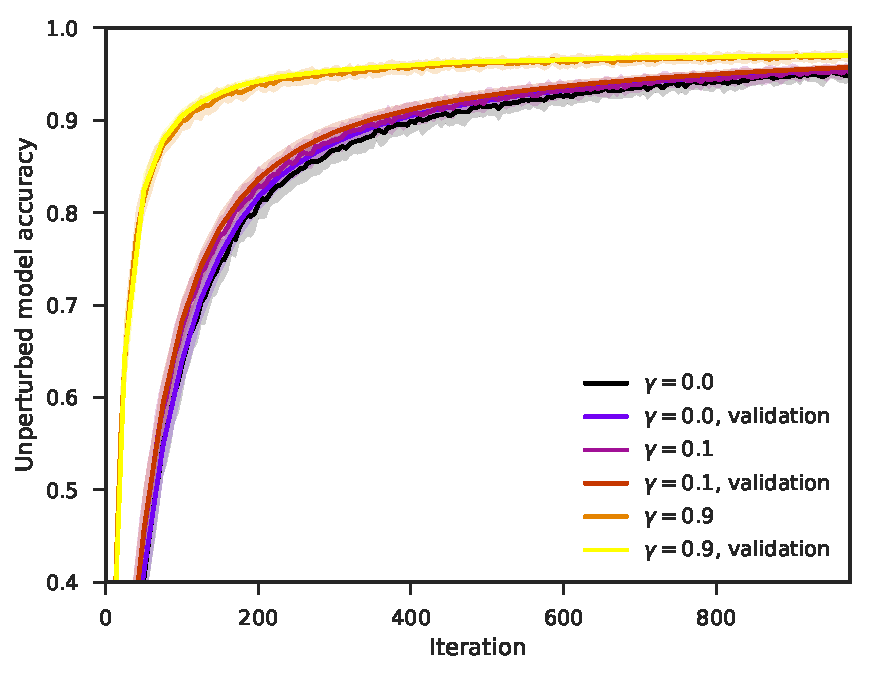
\includegraphics[height=5.8cm]{graphics/E030-MOM-S-analysis/accuracy_unp-all-series-mean-sd.pdf}
%         \caption{}
%         \label{fig: Theory: E030-MOM-S-analysis/accuracy_unp-all-series-mean-sd}
%     \end{subfigure}
%     \hfill
%     \begin{subfigure}[b]{0.49\textwidth}
%         \centering
%         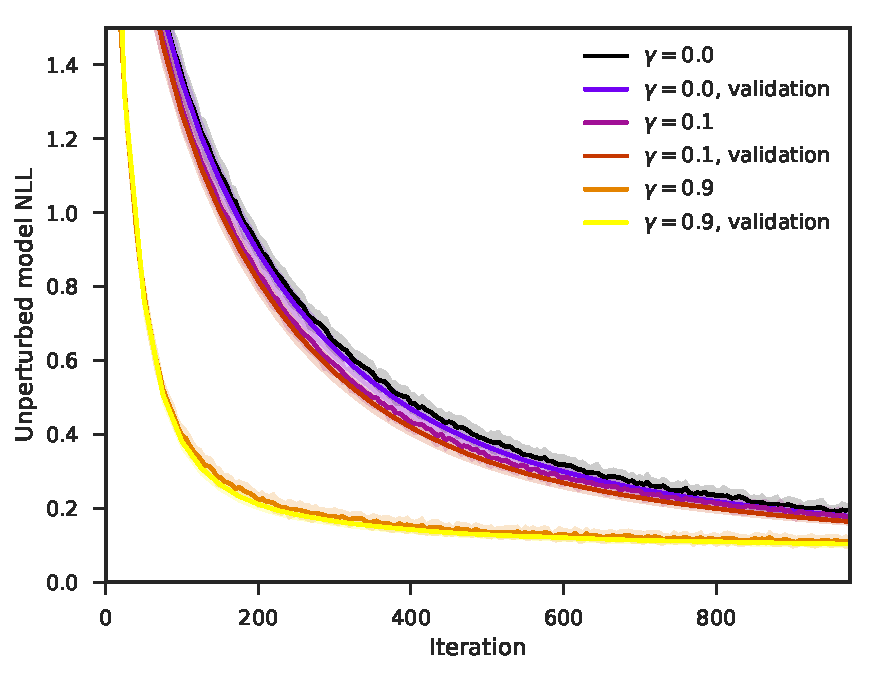
\includegraphics[height=5.8cm]{graphics/E030-MOM-S-analysis/return_unp-all-series-mean-sd.pdf}
%         \caption{}
%         \label{fig: Theory: E030-MOM-S-analysis/return_unp-all-series-mean-sd}
%     \end{subfigure}
%     \caption{
%         Results of experiments using \gls{SGD} with momentum on the \gls{VO} gradient for the unperturbed model run on \gls{MNIST}.
%         \subref{fig: Theory: E030-MOM-S-analysis/accuracy_unp-all-series-mean-sd} Training and validation set classification accuracy.
%         \subref{fig: Theory: E030-MOM-S-analysis/return_unp-all-series-mean-sd} Training and validation set \gls{NLL} loss.
%     }
%     \label{fig: Theory: E030-MOM-S-analysis}
% \end{figure}






